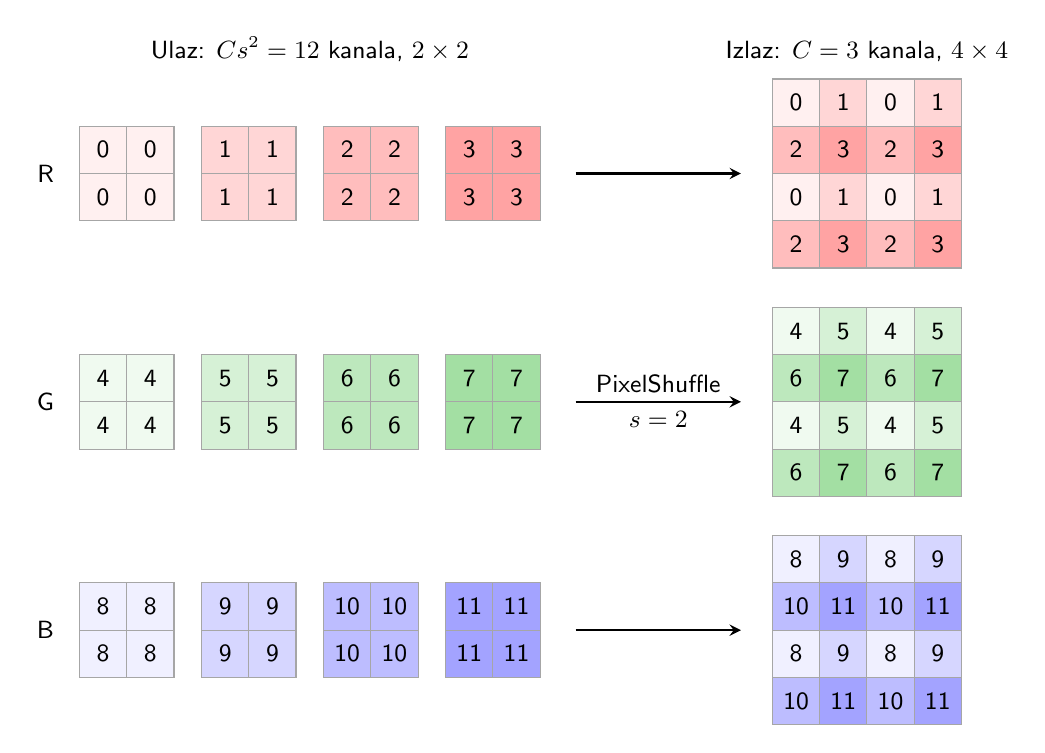
\begin{tikzpicture}[font=\sffamily\small, >=stealth]
	\def\cs{0.6}   % velicina celije
	\def\gap{0.35} % razmak izmedju ulaznih mapa
	\def\row{2.9}  % vertikalni razmak izmedju boja
	\pgfmathsetmacro{\step}{2*\cs+\gap}
	\pgfmathsetmacro{\arx}{4*\step}
	\pgfmathsetmacro{\outx}{\arx+2.6}

	\foreach \c/\col/\name in {0/red/R, 1/green!65!black/G, 2/blue/B} {
		% ulaz: 4 mape 2x2 za kanal boje \c (kanali 4c..4c+3)
		\foreach \i in {0,...,3} {
			\pgfmathtruncatemacro{\k}{4*\c+\i}
			\pgfmathtruncatemacro{\sh}{6+10*\i}
			\begin{scope}[shift={({\i*\step}, {-\c*\row-\cs})}]
				\foreach \x in {0,1} \foreach \y in {0,1}
					\draw[draw=gray!70, fill=\col!\sh] ({\x*\cs}, {-\y*\cs}) rectangle ++(\cs, -\cs);
				\foreach \x in {0,1} \foreach \y in {0,1}
					\node at ({\x*\cs+\cs/2}, {-\y*\cs-\cs/2}) {\k};
			\end{scope}
		}
		\node[anchor=east] at (-0.2, {-\c*\row-2*\cs}) {\name};

		% izlaz: mapa 4x4 za boju \c
		\begin{scope}[shift={(\outx, {-\c*\row})}]
			\foreach \x in {0,...,3} \foreach \y in {0,...,3} {
				\pgfmathtruncatemacro{\idx}{mod(\x,2)+2*mod(\y,2)}
				\pgfmathtruncatemacro{\k}{4*\c+\idx}
				\pgfmathtruncatemacro{\sh}{6+10*\idx}
				\draw[draw=gray!70, fill=\col!\sh] ({\x*\cs}, {-\y*\cs}) rectangle ++(\cs, -\cs);
				\node at ({\x*\cs+\cs/2}, {-\y*\cs-\cs/2}) {\k};
			}
		\end{scope}

		\draw[->, thick] ({\arx+0.1}, {-\c*\row-2*\cs}) -- ++(2.1, 0);
	}

	\node[above] at ({2*\step-\gap/2}, 0.1) {Ulaz: $C s^2 = 12$ kanala, $2\times2$};
	\node[above] at ({\outx+2*\cs}, 0.1) {Izlaz: $C = 3$ kanala, $4\times4$};
	\node[above] at ({\arx+1.15}, {-\row-2*\cs}) {PixelShuffle};
	\node[below] at ({\arx+1.15}, {-\row-2*\cs}) {$s=2$};
\end{tikzpicture}
